% \iffalse
\let\negmedspace\undefined
\let\negthickspace\undefined
\documentclass[journal,12pt,twocolumn]{IEEEtran}
\usepackage{cite}
\usepackage{amsmath,amssymb,amsfonts,amsthm}
\usepackage{algorithmic}
\usepackage{graphicx}
\usepackage{textcomp}
\usepackage{xcolor}
\usepackage{txfonts}
\usepackage{listings}
\usepackage{enumitem}
\usepackage{mathtools}
\usepackage{gensymb}
\usepackage{comment}
\usepackage[breaklinks=true]{hyperref}
\usepackage{tkz-euclide} 
\usepackage{listings}
\usepackage{gvv}                                        
\def\inputGnumericTable{}                                 
\usepackage[latin1]{inputenc}                                
\usepackage{color}                                            
\usepackage{array}                                            
\usepackage{longtable}                                       
\usepackage{calc}                                             
\usepackage{multirow}                                         
\usepackage{hhline}                                           
\usepackage{ifthen}                                           
\usepackage{lscape}

\newtheorem{theorem}{Theorem}[section]
\newtheorem{problem}{Problem}
\newtheorem{proposition}{Proposition}[section]
\newtheorem{lemma}{Lemma}[section]
\newtheorem{corollary}[theorem]{Corollary}
\newtheorem{example}{Example}[section]
\newtheorem{definition}[problem]{Definition}
\newcommand{\BEQA}{\begin{eqnarray}}
\newcommand{\EEQA}{\end{eqnarray}}
\newcommand{\define}{\stackrel{\triangle}{=}}
\theoremstyle{remark}
\newtheorem{rem}{Remark}
\begin{document}
\parindent 0px
\bibliographystyle{IEEEtran}
\title{GATE: CH - 45.2023}
\author{EE22BTECH11219 - Rada Sai Sujan$^{}$% <-this % stops a space
}
\maketitle
\newpage
\bigskip
\section*{Question}
Level \brak{h} in a steam boiler is controlled by manipulating the flow rate \brak{F} of the break-up(fresh) water using a proportional \brak{P} controller. The transfer function between the output and the manipulated input is   \\
$$ \frac{h\brak{s}}{F\brak{s}}=\frac{0.25\brak{1-s}}{s\brak{2s+1}} $$   \\
The measurement and the valve transfer functions are both equal to 1. A process engineer wants to tune the controller so that the closed loop response gives the decaying oscillations under the servo mode. Which one of the following is the CORRECT value of the controller gain to be used by the engineer? \\
\begin{enumerate}
    \item[(A)] $0.25$
    \item[(B)] $2$
    \item[(C)] $4$
    \item[(D)] $6$
\end{enumerate}
\solution
\begin{table}[ht]
    \centering
    \begin{tabular}{|p{2cm}|p{2cm}|p{3.8cm}|}
    \hline
    PARAMETER & VALUE  & DESCRIPTION \\ \hline
    $$G_c$$ & $$K_c$$ & Proportional controller's transfer function \\ \hline
    $$G_f$$ & $$1$$ & Valve transfer function \\ \hline
    $$G_p$$ & $$\frac{0.25\brak{1-s}}{s\brak{2s+1}}$$ & Process transfer function   \\ \hline
    $$G_M$$ & $$1$$ & Measurement transfer function \\ \hline 
    \end{tabular}

    \caption{PARAMETER TABLE 1}
    \label{tab:ch.45.1}
\end{table} \\
Characteristic equation of a second order system can be given by,
\begin{align}
    \tau ^2s^2+2\epsilon \tau s+1 \label{eq:x}
\end{align}
\begin{table}[]
    \centering
    \begin{tabular}{|p{3cm}|p{5cm}|}
    \hline
    PARAMETER & DESCRIPTION   \\ \hline
    $$X\brak{s}$$ & Input signal transfer function  \\ \hline
    $$Y\brak{s}$$ & Output signal transfer function \\ \hline
    $$G\brak{s}$$ & Open loop transfer function    \\ \hline
    $$H\brak{s}$$ & Feedback transfer function    \\ \hline
    $$\tau$$ & Natural time period of oscillation  \\ \hline
    $$\epsilon$$ & Damping coefficient/Damping factor  \\ \hline
    \end{tabular}

    \caption{PARAMETER TABLE 2}
    \label{tab:ch.45.2}
\end{table}
\begin{figure}[ht]
    \centering
    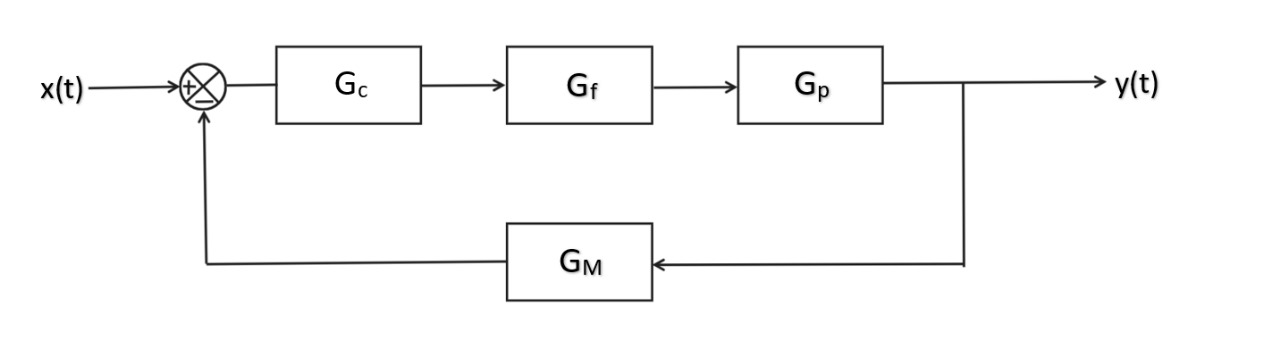
\includegraphics[width=\columnwidth]{figs/block.png}
    \caption{Block diagram}
    \label{fig:ch.45.1}
\end{figure}    \\
Characteristic equation of the above block diagram can be given by,
\begin{align}
     C.H &= 1+G_c G_f G_p G_M   \\
     &= 1+\frac{0.25 K_c \brak{1-s} }{s\brak{2s+1}} 
\end{align}
\begin{align}
    \implies 2s^2+s\brak{1-0.25K_c}+0.25K_c&=0  
\end{align}
Comparing it with the equation \eqref{eq:x},
\begin{align}
    \frac{2}{\tau^2}&=\frac{1-0.25K_c}{2\epsilon \tau}=\frac{0.25K_c}{1}    \\
    \therefore \tau&=\sqrt{\frac{2}{0.25K_c}} , 2\epsilon\tau=\frac{1-0.25K_c}{0.25K_c}
\end{align}
For the system to produce decaying oscillations {$\epsilon <1$},    \\
By verfying options,
\begin{align}
    \therefore \boxed{K_c=2}
\end{align}
\end{document}
